\documentclass[12pt,a4paper]{article}

\usepackage{geometry}
\geometry{
    left=2cm, 
    right=2cm,
    top=3cm,  
    bottom=2cm
}

\usepackage[english,spanish]{babel}
\usepackage[utf8]{inputenc}
\usepackage{amsmath}

\usepackage{graphicx}
\usepackage{wrapfig}
\usepackage{makecell}
\usepackage{booktabs}

\usepackage{setspace}
\setstretch{1.5}
\setlength{\parindent}{0pt}

\usepackage{csquotes}
\usepackage{hyperref}
\usepackage[style=ieee]{biblatex}
\addbibresource{Referencias.bib}

\begin{document}
    \begin{titlepage}
        \begin{minipage}[c]{0.1\textwidth}
            
\includegraphics[width=\textwidth]{./Resources/logo_unam.jpg}
        \end{minipage}
        \begin{minipage}{0.8\textwidth}
            \centering
            {\Large\textbf{Universidad Nacional Autónoma de México}\\}
            {\large\textbf{Escuela Nacional de Estudios Superiores\\\underline{Unidad Morelia}}}
        \end{minipage}
        \begin{minipage}[c]{0.1\textwidth}
            
\includegraphics[width=\textwidth]{./Resources/logo_enes.jpg}
        \end{minipage}
        \vspace{3cm}

        \centering

        {\large{Proyecto Final\\}}
        {\Large\textbf{Predicción del Crecimiento Significativo en Plantas}}
        \vspace{2cm}

        {{PRESENTA:\\}}
        {\large\textbf{Alexis Uriel Aguilar Uribe}}
        \vspace{1cm} 

        {{PROFESORES:\\}}
        {\large\textbf{Dra.\ Marisol Flores Garrido}}\\
        {\large\textbf{Dr.\ Luis Miguel García Velázquez}}
        \vspace{2cm}

        {{GRADO\\}}
        {\large\textbf{Licenciatura en Tecnologías para la Información en Ciencias}}
        \vspace{2cm}

        \flushleft
        {\textbf{Número de Cuenta:\ }424060075}\\
        {\textbf{Asignatura:\ }Sistemas basados en conocimiento [Machine Learning]}
        \vspace{2cm}

        \flushright
        {\textbf{A:\ }\underline{27 de Mayo del 2025}}
        \vfill

    \end{titlepage}

    \tableofcontents
    \newpage

    \section{Introducción}
    {
        En la agricultura, como cualquier otra industria, se vuelve relevante la 
        optimización de los recursos y ganancias, es decir, reducir los insumos 
        consumidos mientras se incrementa la producción (tanto en calidad como en 
        cantidad); todo lo anterior se traduce en aplicar mejoras en diferentes 
        áreas y aspectos que convergen y se relacionan para generar ganancias y 
        reducir costos en la agricultura. Para el caso de este proyecto, el interés 
        se encuentra en el crecimiento de las plantas, bajo qué factores ambientales 
        y de cuidado propician un crecimiento significativo en las plantas.\\ 

        Para lograr el último punto, se tiene como objetivo el crear un modelo de 
        aprendizaje supervisado para la clasificación del crecimiento significativo 
        en base a los factores y mediciones relacionadas a su cuidado y ambiente. 
        Esto se encuentra desarrollado en el repositorio en GitHub dedicado para 
        el proyecto: \href{https://github.com/alexisuaguilaru/Plant_Growth_Model}{Plant Growth Model}.\\
    }
    \newpage

    \section{Descripción de los Datos}
    {
        El conjunto de datos que se emplearán para el proyecto se encuentra disponibles 
        en \cite{dataset_plants}, que es un conjunto de datos publicados en \href{https://www.kaggle.com/}{Kaggle} por 
        la propia comunidad. Se cuenta con siete columnas, donde seis de ellas son 
        atributos y la otra el target, referenciando a la fuente del conjunto de datos, 
        se tienen los siguientes atributos junto con su descripción y tipo de dato: 

        \begin{itemize}
            \item \textbf{Soil\_Type       } [\emph{String}]: El tipo o composición del suelo 
            en el que las plantas están creciendo o se plantan.
            
            \item \textbf{Sunlight\_Hours  } [\emph{Float}]: La duración o intensidad de la luz 
            solar que las plantas reciben.
            
            \item \textbf{Water\_Frequency } [\emph{String}]: Qué tan seguido se riegan las 
            plantas, se indica la frecuencia del riego.
            
            \item \textbf{Fertilizer\_Type } [\emph{String}]: El tipo de fertilizante usado 
            para nutrir a las plantas.
            
            \item \textbf{Temperature      } [\emph{Float}]: Las condiciones de la temperatura 
            ambiental bajo las cuales las plantas están creciendo.

            \item \textbf{Humidity         } [\emph{Float}]: El nivel de humedad en el ambiente 
            alrededor de las plantas.

            \item \textbf{Growth\_Milestone} [\emph{Integer, Target}]: Descripción o marcadores 
            que indican la etapa o eventos significativos en el proceso de crecimiento de 
            las plantas.
        \end{itemize}

        Por último, el conjunto de datos consta de $193$ instancias (filas), las diferentes 
        instancias lucen de la siguiente manera:

        \begin{center}    
            \begin{tabular}{lrll}
                \toprule
                Soil\_Type & Sunlight\_Hours & Water\_Frequency & Fertilizer\_Type \\
                \midrule
                sandy & 9.228 & daily     & none     \\
                sandy & 9.774 & weekly    & chemical \\
                clay  & 7.392 & bi-weekly & none     \\
                clay  & 6.462 & bi-weekly & organic  \\
                clay  & 8.846 & weekly    & organic  \\
                loam  & 5.985 & bi-weekly & chemical \\
                \bottomrule
            \end{tabular}
            \begin{tabular}{rrr}
                \toprule
                Temperature & Humidity & Growth\_Milestone \\
                \midrule
                33.804 & 32.815 & 0 \\
                32.549 & 61.377 & 1 \\
                31.100 & 68.600 & 0 \\
                27.517 & 34.175 & 1 \\
                27.700 & 56.800 & 1 \\
                29.757 & 57.476 & 0 \\
                \bottomrule
            \end{tabular}
        \end{center}

    }
    \newpage

    \section{Análisis Exploratorio de Datos}
    {
        Los tipos de datos en base a la descripción proporcionada en \cite{dataset_plants} 
        con la mostrada al momento de la lectura de los datos en Python, por lo que no 
        es necesario realizar una transformación sobre los tipos de datos de cada atributo. \\
        
        Debido a que los valores que toma y representan el target, \emph{Growth\_Milestone}, 
        son enteros, se tiene que el modelo que se generará será un clasificador binario; cuyas clases 
        representan si hay un crecimiento significativo, bajo ciertos criterios, en las plantas. 
        Como primera observación se tiene que el conjunto de datos está balanceado respecto 
        a las clases, por lo que se podría usar cualquiera de las métricas bajo una 
        justificación válida o apropiada al problema:

        \begin{center}
            \begin{tabular}{lr}
            \toprule
                Growth\_Milestone &  \\
                Clases & Conteo \\
            \midrule
                0 [No Milestone] & 97 \\
                1 [Milestone] & 96 \\
            \bottomrule
            \end{tabular}
        \end{center}
        
        Se presenta un análisis univariado sobre los atributos numéricos y categóricos, y 
        por último se prueban algunas hipótesis relevantes y relacionadas sobre las observaciones 
        en los apartados anteriores.\\

        \subsection{Atributos Numéricos}
        {
            Generando la descriptiva básica (medidas centrales y de dispersión) de 
            los datos se obtienen los siguientes resultados:

            \begin{center}
                \begin{tabular}{lrrr}
                \toprule
                    Medida & Sunlight\_Hours & Temperature & Humidity \\
                \midrule
                    Media               & 6.8264 & 25.0760 & 58.0989 \\
                    Desviación Estándar & 1.5995 &  5.3541 & 12.6317 \\
                    Mínimo              & 4.0331 & 15.2000 & 30.5676 \\
                    $Q_1$               & 5.4770 & 20.6370 & 49.3000 \\
                    $Q_2$               & 6.8332 & 25.9123 & 59.1828 \\
                    $Q_3$               & 8.2411 & 29.7579 & 69.1000 \\
                    Máximo              & 9.9139 & 34.8101 & 79.6482 \\
                \bottomrule
                \end{tabular}
            \end{center}

            Primero se destaca que siguen diferentes rangos de valores, por lo que se 
            tendrán que estandarizar o blanquear para su adecuado uso para el entrenamiento 
            de los modelos que se crearán, además de permitir realizar comparativas entre 
            las distribuciones. Al estandarizar los valores se tienen los siguientes resultados:

            \begin{center}
                \begin{tabular}{lrrr}
                \toprule
                Medida & Sunlight\_Hours & Temperature & Humidity \\
                \midrule
                Media               & 0 & 0 & 0 \\
                Desviación Estándar & 1 & 1 & 1 \\
                Mínimo              & -1.746 & -1.8445 & -2.1795 \\
                $Q_1$               & -0.843 & -0.8290 & -0.6965 \\
                $Q_2$               &  0.004 &  0.1561 &  0.0858 \\
                $Q_3$               &  0.884 &  0.8744 &  0.8709 \\
                Máximo              &  1.930 &  1.8180 &  1.7059 \\
                \bottomrule
                \end{tabular}
            \end{center}

            Destacándose que el atributo \emph{Sunlight\_Hours} figura que sigue una 
            distribución debido a que su $Q_2$ se aproxima a $0$ junto que sus $Q_1$ 
            y $Q_3$ se parecen, salvo el signo. Mientras que en \emph{Humidity} su $Q_2$ 
            se encuentra equidistante a $Q_1$ y a $Q_3$, lo que significa que no tiene 
            sesgo más no es simétrica. Y en \emph{Temperature}, por sus cuartiles, tiene 
            un sesgo negativo considerable. En base a lo mencionado se tiene que los tres 
            atributos siguen diferentes distribuciones, implicando que estos atributos surgen 
            de diferentes fenómenos, interacciones y procesos que impactan en el crecimiento 
            de las plantas, por lo que los tres atributos se vuelven relevantes para la 
            clasificación debido a que cada uno condensa diferentes procesos para lograr un 
            crecimiento significativo.\\

            De los box plots, se puede observar que las distribuciones de los atributos 
            no son tan diferentes según el target, según si hay un crecimiento significativo, 
            esto al ver que las cajas están superpuestas, haciendo que no exista una diferencia 
            Significativa entre las medias de las distribuciones. Lo que se destaca es que 
            cuando existe un crecimiento significativo tiende a tomar valores más bajos y además 
            de que su desviación estándar también tiende a decrecer.\\ 

            Este último hecho se podría relacionar con que existe un control sobre los factores 
            ambientales, haciendo que las distribuciones sean más restrictivas y reguladas, 
            dejando afuera posibles fenómenos que generen un ambiente irregular para el 
            crecimiento de las propias plantas. Haciendo que la planta esté en un ambiente ideal 
            para su crecimiento pero, por las distribuciones, existe la posibilidad de que aunque 
            esté en las condiciones idóneas no logre un crecimiento significativo.

            \begin{center}
                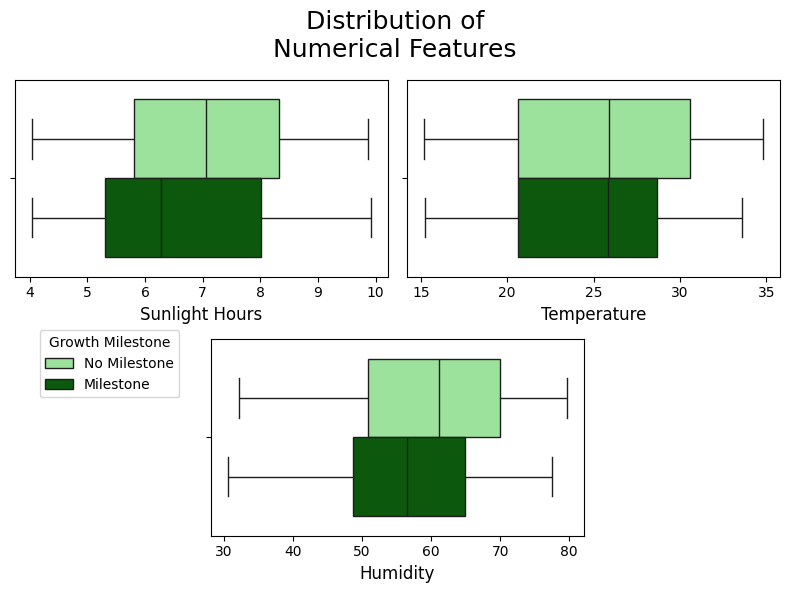
\includegraphics[width=0.85\textwidth]{./Resources/3_1.png}
            \end{center}

            De manera visual, no se cuenta con valores atípicos derivados de la Regla del 
            Rango Intercuartil ni valores faltantes, por lo que estos atributos numéricos se 
            encuentran preparados para la fase de entrenamiento.
        }

    }
    \newpage

    \section{Metodología del Proyecto}
    {}
    \newpage

    \section{Experimentos y Discusión de Resultados}
    {}
    \newpage

    \section{Análisis de los Resultados}
    {}
    \newpage

    \section{Conclusiones}
    {}
    \newpage

    \printbibliography[heading=bibintoc,title={Referencias Bibliográficas}]

\end{document}